\documentclass{article}

% NeurIPS 2026 style. Download neurips_2026.sty from
% https://neurips.cc/Conferences/2026/CallForPapers and put it beside this file.
% Submission is ANONYMOUS: do not pass [final].
\usepackage{neurips_2026}

\usepackage[utf8]{inputenc}
\usepackage[T1]{fontenc}
\usepackage{hyperref}
\usepackage{url}
\usepackage{booktabs}
\usepackage{amsfonts}
\usepackage{amsmath}
\usepackage{nicefrac}
\usepackage{microtype}
\usepackage{graphicx}
\usepackage{xcolor}

\graphicspath{{figs/}}

% Placeholder for numbers awaiting a training run. Remove this macro (and every
% use of it) before submitting -- if a \TODO survives to the PDF, that number was
% never measured.
\newcommand{\TODO}[1]{\textcolor{red}{\textbf{[TODO: #1]}}}

\title{The Variational Sparse Autoencoder is an $L_2$ Penalty:\\
Feature Death and Metric Artifacts in Gaussian-Prior SAEs}

\author{Anonymous Author(s)\\Affiliation\\\texttt{email}}

\begin{document}
\maketitle

\begin{abstract}
Variational sparse autoencoders (vSAEs) are motivated by the hope that a
probabilistic latent space organises features more coherently than a
deterministic one. We show that the standard construction does not test this
hypothesis. A vSAE with an isotropic Gaussian prior and fixed unit variance
degenerates \emph{exactly} into a TopK SAE with an $L_2$ penalty on its
activations: the KL term collapses to $\tfrac{1}{2}\|\boldsymbol{\mu}\|^2$, the
reparameterisation trick becomes a no-op, and no sample is ever drawn. We verify
this degeneracy in a public vSAE implementation and then characterise what the
residual $L_2$ penalty does. Holding architecture, sparsity, and dead-feature
revival fixed, the fraction of live features falls monotonically from $78\%$ to
$35\%$ as the KL coefficient $\beta$ sweeps $10^{-4}$ to $10^{2}$, while
activation scale collapses by $8\times$ --- the signature of shrinkage, not of
dispersion. Critically, this shrinking dictionary is rewarded by two widely used
SAEBench metrics: the vSAE outscores its baseline on spurious correlation removal
and targeted probe perturbation while using a fraction of the live features, so
these apparent wins track dictionary size rather than feature quality. We argue
that claims about variational SAEs require two controls that are currently absent
from the literature: a plain $L_2$ activation penalty, and a size-matched
dictionary.
\end{abstract}

\section{Introduction}

Sparse autoencoders (SAEs) decompose language model activations into an
overcomplete dictionary of sparse, putatively monosemantic
features~\citep{sharkey2022taking,cunningham2023sparse,bricken2023monosemanticity},
motivated by the observation that features are represented in
superposition~\citep{elhage2022superposition}.
A natural extension is to make the latent code probabilistic, as in the
variational autoencoder~\citep{kingma2013autoencoding}. The intuition is
appealing and frequently stated: sampling turns each feature from a point into a
region, and the resulting overlap penalty should push features apart, yielding a
better-organised dictionary. We set out to test this hypothesis and found that,
as standardly constructed, it cannot be tested at all.

Our contributions:

\begin{itemize}
\item \textbf{A degeneracy result} (\S\ref{sec:degeneracy}). With an isotropic
Gaussian prior and the fixed unit variance used in practice, the vSAE objective
reduces to a TopK SAE with an $L_2$ activation penalty. The stochastic component
is inert: no noise is sampled in either training or inference. Any behaviour
attributed to ``variational structure'' in such a model is attributable to the
penalty instead.

\item \textbf{A dose-response characterisation of the penalty}
(\S\ref{sec:death}). Sweeping $\beta$ over six orders of magnitude with all else
held fixed --- including the auxiliary dead-feature revival loss --- live features
fall monotonically and near-linearly in $\log\beta$, and activation magnitude
collapses. This is what an activation penalty predicts and what a dispersive force
does not.

\item \textbf{A measurement-validity warning} (\S\ref{sec:artifact}). The vSAE
outperforms its baseline on SCR and TPP while holding far fewer live features.
Because both metrics reward ablations that are selective, they improve as a
dictionary shrinks. We argue these scores cannot be read as evidence of
disentanglement without a size-matched control, and report one.
\end{itemize}

We regard this as a cautionary result about experimental design rather than a
verdict on probabilistic sparse coding. A Gaussian prior is a poor prior for a
sparse code --- it places no mass at zero, and its KL is pure shrinkage --- so its
failure says little about priors that do.

\section{The Gaussian vSAE degenerates to an $L_2$ penalty}
\label{sec:degeneracy}

\paragraph{Baseline.} A TopK SAE~\citep{gao2024scalingevaluatingsparseautoencoders}
encodes activations $\mathbf{x}\in\mathbb{R}^d$ as
$\mathbf{f}=\mathrm{ReLU}(\mathbf{W}_{\mathrm{enc}}\mathbf{x}+\mathbf{b}_{\mathrm{enc}})$,
keeps the $K$ largest entries, and decodes
$\hat{\mathbf{x}}=\mathbf{W}_{\mathrm{dec}}\mathbf{f}_{\mathrm{topk}}+\mathbf{b}_{\mathrm{dec}}$.
Sparsity is architectural, so the objective carries no $L_1$ term:
\begin{equation}
\mathcal{L}_{\mathrm{SAE}} = \|\mathbf{x}-\hat{\mathbf{x}}\|_2^2
+ \alpha\,\mathcal{L}_{\mathrm{aux}},
\label{eq:sae}
\end{equation}
where $\mathcal{L}_{\mathrm{aux}}$ is the AuxK loss that revives dead features by
asking the top $k_{\mathrm{aux}}$ dead latents to explain the residual.

\paragraph{Variational version.} The vSAE treats the code as a posterior
$q(\mathbf{z}\mid\mathbf{x})=\mathcal{N}(\boldsymbol{\mu},\boldsymbol{\sigma}^2)$
with $\boldsymbol{\mu}$ produced by the encoder, samples via
$\mathbf{z}=\boldsymbol{\mu}+\boldsymbol{\epsilon}\odot\boldsymbol{\sigma}$,
applies TopK to $\mathbf{z}$, and regularises toward $p(\mathbf{z})=\mathcal{N}(\mathbf{0},\mathbf{I})$:
\begin{equation}
\mathcal{L}_{\mathrm{vSAE}} = \|\mathbf{x}-\hat{\mathbf{x}}\|_2^2
+ \beta\,\mathrm{KL}\!\left[q(\mathbf{z}\mid\mathbf{x})\,\|\,p(\mathbf{z})\right]
+ \alpha\,\mathcal{L}_{\mathrm{aux}}.
\label{eq:vsae}
\end{equation}

The coefficient $\beta$ plays the same role as in $\beta$-VAE~\citep{higgins2017betavae},
where it trades reconstruction against the strength of the prior.

\paragraph{The collapse.} Implementations fix $\boldsymbol{\sigma}=\mathbf{1}$ for
stability and memory. Two things follow. First, the KL loses its variance terms,
\begin{equation}
\mathrm{KL}\!\left[\mathcal{N}(\boldsymbol{\mu},\mathbf{I})\,\|\,\mathcal{N}(\mathbf{0},\mathbf{I})\right]
= \tfrac{1}{2}\textstyle\sum_i \left(\mu_i^2 + 1 - 1 - \log 1\right)
= \tfrac{1}{2}\|\boldsymbol{\mu}\|_2^2 ,
\label{eq:kl}
\end{equation}
which is an $L_2$ penalty on the pre-activation. Second --- and this is the part
that is easy to miss --- when the variance is a fixed constant rather than a
learned function of $\mathbf{x}$, there is no posterior to sample from that
carries information, and implementations gate the sampling step off entirely. In
the implementation we study, the encoder computes
$\boldsymbol{\mu}=\mathrm{ReLU}(\mathbf{W}_{\mathrm{enc}}\mathbf{x}+\mathbf{b}_{\mathrm{enc}})$
and the latent is assigned $\mathbf{z}=\boldsymbol{\mu}$ whenever the
learned-variance flag is off, which is the setting used for every released
checkpoint. Substituting into Eq.~\ref{eq:vsae}:
\begin{equation}
\mathcal{L}_{\mathrm{vSAE}} \;=\; \|\mathbf{x}-\hat{\mathbf{x}}\|_2^2
\;+\; \frac{\beta}{2}\,\|\mathbf{f}\|_2^2 \;+\; \alpha\,\mathcal{L}_{\mathrm{aux}},
\qquad \mathbf{f}=\mathrm{ReLU}(\mathbf{W}_{\mathrm{enc}}\mathbf{x}+\mathbf{b}_{\mathrm{enc}}),
\label{eq:degenerate}
\end{equation}
which is Eq.~\ref{eq:sae} plus an $L_2$ activation penalty. The encoder, the
sparsity mechanism, and the decoder are unchanged. The reparameterisation trick,
the posterior, and the prior have all vanished.

This matters because the dispersive-pressure hypothesis is a claim about
\emph{sampling}: features are supposed to repel because their sampled regions
overlap. Under Eq.~\ref{eq:degenerate} nothing is sampled, so the hypothesis is
not merely unsupported --- it is untested. In \S\ref{sec:death} we show what the
surviving penalty actually does.

\section{Experimental setup}
\label{sec:setup}

We train TopK SAEs and Gaussian vSAEs on residual stream activations using a
modified \texttt{dictionary\_learning} framework~\citep{marks2024dictionary_learning},
evaluate with SAEBench~\citep{karvonen2025saebenchcomprehensivebenchmarksparse},
and measure feature usage by streaming $10^6$ activations and recording, for each
dictionary element, whether it is ever selected by TopK. A feature is
\emph{live} if it is selected at least once.

Two settings are used. The \textbf{$\beta$ sweep} (\S\ref{sec:death}) uses a
1-layer GeLU transformer, \texttt{blocks.0.hook\_resid\_post}, $d_{\mathrm{model}}=512$,
dictionary size $2048$ ($4\times$), $K=256$, AuxK $\alpha=1/32$, learning rate
$8\times10^{-4}$, $10{,}000$ steps, bfloat16. Only $\beta$ varies. The
\textbf{benchmark comparison} (\S\ref{sec:artifact}) uses Pythia-70M-deduped,
\texttt{blocks.3.hook\_resid\_post}, dictionary size $8192$ ($16\times$), $K=256$.
Training data is TinyStories~\citep{eldan2023tinystoriessmalllanguagemodels} with
128-token contexts. All runs used a single RTX 3080.

\section{The penalty kills features, monotonically in $\beta$}
\label{sec:death}

If Eq.~\ref{eq:degenerate} is right, $\beta$ is a shrinkage knob. Shrinking
pre-activations pushes marginal features below the TopK threshold; once a feature
stops being selected it receives no reconstruction gradient, and only AuxK can
revive it. The prediction is a monotonic loss of live features in $\beta$,
accompanied by a collapse in activation magnitude. Dispersion predicts neither.

\begin{figure}[t]
\centering
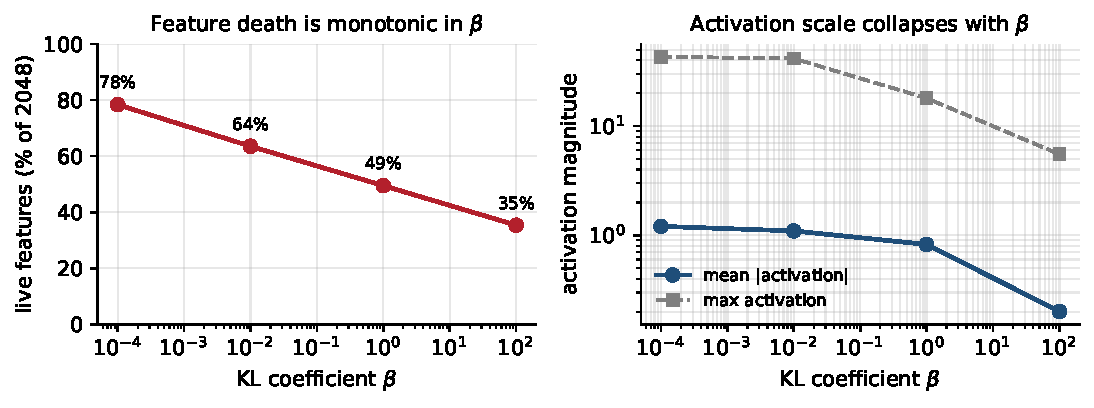
\includegraphics[width=\textwidth]{beta_sweep.pdf}
\caption{Sweeping the KL coefficient with everything else fixed (1-layer GeLU,
$d{=}2048$, $K{=}256$, AuxK $\alpha{=}1/32$, $10^6$ evaluation activations).
\textbf{Left:} live features fall monotonically and near-linearly in $\log\beta$,
roughly $14$ percentage points per decade. \textbf{Right:} mean and maximum
activation magnitude collapse, the maximum by $8\times$. Both are signatures of
shrinkage on the code.}
\label{fig:sweep}
\end{figure}

\begin{table}[t]
\centering
\caption{The $\beta$ dose-response. AuxK dead-feature revival is \emph{active and
identical} at every point, so the loss of features is not an absence of
mitigation.}
\label{tab:sweep}
\begin{tabular}{lcccc}
\toprule
$\beta$ & live features / 2048 & \% live & mean activation & max activation \\
\midrule
$10^{-4}$ & 1605 & 78.4 & 1.209 & 43.12 \\
$10^{-2}$ & 1301 & 63.5 & 1.097 & 41.59 \\
$10^{0}$  & 1013 & 49.5 & 0.825 & 18.01 \\
$10^{2}$  &  724 & 35.4 & 0.201 & \phantom{0}5.53 \\
\bottomrule
\end{tabular}
\end{table}

Table~\ref{tab:sweep} and Figure~\ref{fig:sweep} confirm the prediction. Live
features decline monotonically across six orders of magnitude of $\beta$, and the
decline is close to linear in $\log\beta$. Activation scale falls in step: the
largest activation observed over $10^6$ tokens drops from $43.1$ to $5.5$. The
strongest control here is that AuxK is enabled with the same coefficient at every
point, so this is not a failure to apply the standard dead-feature remedy --- it is
death that occurs despite it.

\paragraph{An interventional test.} The account above makes a sharper, falsifiable
prediction. Under Eq.~\ref{eq:degenerate} the penalty applies to \emph{all}
dictionary entries, including those TopK did not select; unselected features are
therefore shrunk without ever receiving reconstruction gradient to push back. If
we mask the penalty to the selected features only, feature death should largely
disappear. We train an otherwise identical model with the KL restricted to the
TopK-selected coordinates and find \TODO{masked-KL live features, vs. 1013
unmasked at $\beta{=}1$}. \TODO{one sentence stating whether this confirms or
refutes the mechanism}

\paragraph{Does real sampling change the picture?} Because
Eq.~\ref{eq:degenerate} applies only when the variance is fixed, we also train a
model with a learned per-feature variance, in which the reparameterisation trick
is genuinely active. \TODO{learned-variance live features and learned $\sigma$
behaviour, vs. 1013 fixed-variance}. \TODO{state whether the posterior collapses
toward determinism, which would indicate the degeneracy is the optimum rather
than an implementation choice}

\section{Benchmark ``wins'' track dictionary size}
\label{sec:artifact}

On Pythia-70M the vSAE is slightly worse than the TopK baseline on core
reconstruction metrics --- cross-entropy loss and explained variance --- and holds
dramatically fewer live features: $1474$ of $8192$ ($18.0\%$) against the
baseline's $7379$ ($90.1\%$).

Yet on two SAEBench metrics the vSAE \emph{wins}. Spurious Correlation Removal
(SCR), adapted from SHIFT~\citep{marks2025sparsefeaturecircuitsdiscovering},
measures how cleanly task-irrelevant concepts can be ablated while preserving
accuracy. Targeted Probe Perturbation (TPP) measures whether ablating the latents
for one class degrades that class without disturbing others. The vSAE scores
higher on both, peaking at higher thresholds, and degrades more gracefully.

The preprint version of this work read these as evidence of a more disentangled
latent space. We now think that reading is unsafe, for a structural reason: both
metrics reward \emph{selectivity} of ablation, and selectivity is easier to
achieve with fewer live features. A dictionary with $18\%$ of its entries alive
has fewer opportunities for an ablation to touch an unintended concept. The metric
improves for a reason that has nothing to do with the quality of the features that
remain. Dictionary size is a confounder for SCR and TPP, and it is not routinely
controlled.

\paragraph{A size-matched control.} We test this directly by restricting the
trained baseline SAE to its $1474$ most-frequently-selected features --- matching
the vSAE's live count without retraining or changing any feature --- and re-running
SCR and TPP. \TODO{size-matched SAE SCR/TPP scores vs. full SAE and vs. vSAE}.
\TODO{one sentence: if the size-matched baseline improves toward the vSAE, the
win is a size artifact; if not, the vSAE has genuinely better-separated features}

\paragraph{A confound in our own comparison.} The $1474$ vs.\ $7379$ figure
overstates the effect, and we report it with that caveat. The baseline was trained
with AuxK revival at $\alpha=1/32$; the vSAE checkpoint was trained with
$\alpha=0$. The comparison therefore conflates the KL penalty with the absence of
the standard dead-feature remedy. We retrain the vSAE with AuxK enabled and obtain
\TODO{live features with AuxK on, out of 8192}. The $\beta$ sweep in
\S\ref{sec:death} is not affected: AuxK is held at $1/32$ throughout it, so the
mechanism claim rests on the controlled experiment rather than on this comparison.

\section{Discussion}

\paragraph{What we did and did not show.} We showed that a specific and widely
natural construction --- isotropic Gaussian prior, fixed unit variance --- is not
variational in any operative sense, and that the $L_2$ penalty it reduces to
destroys dictionary capacity in a smooth, predictable way. We did \emph{not} show
that probabilistic sparse coding is unpromising. A Gaussian prior is arguably the
worst available choice for a sparse code: it has no mass at zero, so it cannot
express ``this feature is usually off,'' and its KL is exactly the shrinkage that
causes the damage we measure. Priors built for sparsity --- spike-and-slab,
Laplace --- have the qualitative property a sparse code needs, and are untested
here. The mechanism we identify is what tells us where to look next.

\paragraph{Implications for evaluation.} Our central practical claim is a
methodological one. A vSAE result is uninterpretable without two controls that are
cheap and currently uncommon: (i) a TopK SAE trained with an explicit $L_2$
activation penalty of matched strength, which under Eq.~\ref{eq:degenerate} should
reproduce the fixed-variance vSAE to within noise; and (ii) a dictionary-size
matched baseline whenever SCR, TPP, or any other ablation-selectivity metric is
reported. Without (i), ``variational'' credit accrues to a penalty. Without (ii),
metric improvements accrue to a shrinking dictionary. Both failure modes are
invisible in the aggregate scores, and both produce results that look like
progress.

\paragraph{Limitations.} We study one architecture family (TopK), two small models,
one layer each, and a single dataset. Live-feature counts depend on the evaluation
corpus, and a feature never selected on TinyStories may be selected elsewhere. The
degeneracy of Eq.~\ref{eq:degenerate} is a property of the fixed-variance
construction and does not apply to learned-variance vSAEs, gated variational
schemes such as VSEase~\citep{lu2025sparseautoencodersagain}, or approaches that
place the stochasticity outside the sparsity mechanism.

\bibliographystyle{plainnat}
\bibliography{references}

\end{document}
